\chapter{\label{chap:results}Results and Findings}

This chapter presents the results of the GC detection applied across the areas described in Chapter~{\ref{chap:data}}. They consist of a number of tables and plots which correspond to:
\begin{enumerate}
    \item The three stages of the pipeline:
          \begin{enumerate}[label=\roman*.]
              \item Raster Exclusion Using \blobdog{} (in Section~{\ref{sec:results-DoG}})
              \item Ant Colony (in Section~\ref{sec:results-ant})
              \item Gravitational Clustering (in Section~\ref{sec:results-clustering})
          \end{enumerate}
    \item The full pipeline (in Section~\ref{sec:results-pipeline})
\end{enumerate}

Note that each stage of the pipeline may depend on the results from the previous stages. Thus, the parametric variation that provides the best results for a given stage is carried forward as the basis for the future stages of the pipeline.

\section{\label{sec:results-DoG}Raster Exclusion Using \blobdog{}}

To determine a sufficient value for $B_{\text{threshold}}$, the \blobdog{} filter was run across all rasters for all areas while varying the threshold. Table~\ref{tb:number-of-remaining-rasters} shows the number of rasters that remained in each area for the different threshold values.

\begin{table}[H]
    \centering
    \caption{Rasters Remaining After the Execution of \blobdog{} for Various Values of $B_{\text{threshold}}$}
    \label{tb:number-of-remaining-rasters}
    \begin{tabular}{l c@{\hspace{1.0\tabcolsep}}c c@{\hspace{1.0\tabcolsep}}c c@{\hspace{1.0\tabcolsep}}c c@{\hspace{1.0\tabcolsep}}c c@{\hspace{1.0\tabcolsep}}c c@{\hspace{1.0\tabcolsep}}c c@{\hspace{1.0\tabcolsep}}c}
        \toprule
        Area                                               & \multicolumn{12}{C{8cm}}{Number of Rasters Remaining (All~Rasters~\&~Rasters~Containing~Known~GCs)} & \multicolumn{2}{C{1.65cm}}{Total Number of Rasters}                                                                                                                                                                                                                                 \\
        \midrule{}
                                                           & \multicolumn{12}{c}{$B_{\text{threshold}}$}                                                         & \multicolumn{2}{c}{}                                                                                                                                                                                                                                                                \\
        \cmidrule(lr){2-13}
                                                           & \multicolumn{2}{c}{$0.1$}                                                                           & \multicolumn{2}{c}{$0.2$\footnotemark{}}            & \multicolumn{2}{c}{$0.3$} & \multicolumn{2}{c}{$0.4$} & \multicolumn{2}{c}{$0.5$} & \multicolumn{2}{c}{$0.6$} &             &                                                                                                 \\
        \midrule
                                                           & {\tiny All}                                                                                         & {\tiny GCs}                                         & {\tiny All}               & {\tiny GCs}               & {\tiny All}               & {\tiny GCs}               & {\tiny All} & {\tiny GCs} & {\tiny All} & {\tiny GCs} & {\tiny All} & {\tiny GCs} & {\tiny All} & {\tiny GCs} \\
        Area 1                                             & 512                                                                                                 & 12                                                  & 8                         & 7                         & 8                         & 7                         & 7           & 7           & 7           & 7           & 7           & 7           & 512         & 12          \\
        Area 2: $\SI{2.0}{\degree}\times\SI{2.0}{\degree}$ & 35                                                                                                  & 1                                                   & 28                        & 1                         & 10                        & 1                         & 7           & 1           & 3           & 1           & 2           & 1           & 35          & 1           \\
        Area 2: $\SI{4.0}{\degree}\times\SI{4.0}{\degree}$ & 12                                                                                                  & 1                                                   & 9                         & 1                         & 8                         & 1                         & 7           & 1           & 7           & 1           & 5           & 1           & 12          & 1           \\
        Area 3                                             & 285                                                                                                 & 12                                                  & 39                        & 11                        & 29                        & 10                        & 19          & 9           & 18          & 9           & 16          & 9           & 285         & 12          \\
        Area 4                                             & 120                                                                                                 & 0                                                   & 60                        & 0                         & 10                        & 0                         & 9           & 0           & 6           & 0           & 4           & 0           & 120         & 0           \\
        \midrule
        Total                                              & 964                                                                                                 & 26                                                  & 144                       & 20                        & 65                        & 19                        & 58          & 18          & 41          & 18          & 34          & 18          & 964         & 26          \\
        \bottomrule
    \end{tabular}
\end{table}
\footnotetext{This was the threshold that was used for the future stages of the pipeline.}

When the threshold is set too low one or more blobs are detected in every raster (as is the case with $B_{\text{threshold}} = 0.1$). As this value increases the number of blobs detected in each area is reduced. For these various thresholds $B_{\text{threshold}} = 0.2$ provides the largest reduction in the number of rasters while still maintaining the most of the rasters that contain known GCs. Thus, this threshold is selected as the basis for the future steps of the pipeline. The results of applying \blobdog{} with this threshold  across each area may be seen in Figure~\ref{fig:filtered-dog-rasters}. This presents the rasters that are kept for this threshold and highlights which GCs are among those kept and among those removed.

\begin{figure}[H]
    \centering
    \begin{subfigure}[b]{0.75\textwidth}
        \includegraphics[width=\textwidth, height=6cm]{rasters/overlay/area-1-dog.pdf}
        \caption{\label{fig:dog-a1-overview}Area 1}
    \end{subfigure}

    \begin{subfigure}[b]{0.49\textwidth}
        \includegraphics[width=\textwidth, height=6cm]{rasters/overlay/area-2-dog.pdf}
        \caption{\label{fig:dog-a2-overview}Area 2: $\SI{2.0}{\degree}\times\SI{2.0}{\degree}$}
    \end{subfigure}
    \begin{subfigure}[b]{0.49\textwidth}
        \includegraphics[width=\textwidth, height=6cm]{rasters/overlay/area-2-4x4dog.pdf}
        \caption{\label{fig:dog-a2-4x4-overview}Area 2: $\SI{4.0}{\degree}\times\SI{4.0}{\degree}$}
    \end{subfigure}

    \begin{subfigure}[b]{0.49\textwidth}
        \includegraphics[width=\textwidth, height=6cm]{rasters/overlay/area-3-dog.pdf}
        \caption{\label{fig:dog-a3-overview}Area 3}
    \end{subfigure}
    \begin{subfigure}[b]{0.49\textwidth}
        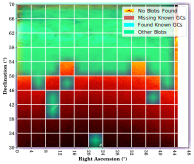
\includegraphics[width=\textwidth, height=6cm]{rasters/overlay/area-4-dog.pdf}
        \caption{\label{fig:dog-a4-overview}Area 4}
    \end{subfigure}
    \caption{\label{fig:filtered-dog-rasters}\blobdog{} Raster Classification with $B_{\text{threshold}} = 0.2$}
\end{figure}

Each area in this figure is represented as a raster plot where \blobdog{} finds \textit{known GCs}, \textit{other blobs} (corresponding to other stellar structures such as galaxies, dwarf galaxies, and open clusters), and \textit{no blobs}. In these plots, rasters containing known GCs that were not maintained by \blobdog{} (\textit{missing known GCs}) are also highlighted. To provide a clear depiction of where these blobs are located, the results have been overlaid on the stellar distribution heat-map for each area.

It is evident that rasters in regions with a high number of stars or regions with a large variation in their stellar density have blobs detected by \blobdog{}. Figure~\ref{fig:dog-a2-overview} and \ref{fig:dog-a2-4x4-overview} depicting Area 2 and~\ref{fig:dog-a4-overview} depicting Area 4 find blobs mainly at the bright dense regions within those areas. Area 3 represented by Figure~\ref{fig:dog-a3-overview} has most of its blobs detected at the locations of the Magellanic Clouds. Additionally, the dark regions within this area have no blobs detected except in the one raster that contains a known GC. Area 1 finds blobs mainly around the GCs, but does not seem to find any blobs in the brightest regions in the corners of Figure~\ref{fig:dog-a1-overview}.

Table~\ref{tb:areas-found-rasters-0.2} lists the GCs present across the areas and specifies whether the raster they are contained within was maintained by \blobdog{}.

\begin{table}[H]
    \centering
    \caption{Known GCs detected at $B_{\text{threshold}} = 0.2$}
    \label{tb:areas-found-rasters-0.2}
    \begin{tabular}{l@{\hspace{0.1\tabcolsep}}C{0.15\linewidth}l@{\hspace{0.1\tabcolsep}}C{0.15\linewidth}l@{\hspace{0.1\tabcolsep}}C{0.15\linewidth}}
        \toprule
        \multicolumn{2}{c}{Area 1} & \multicolumn{2}{c}{Area 2} & \multicolumn{2}{c}{Area 3}                                                                          \\
        \cmidrule(lr){1-2} \cmidrule(lr){3-4} \cmidrule(lr){5-6}
        GC                         & Present After \blobdog{}?  & GC                         & Present After \blobdog{}? & GC           & Present After \blobdog{}?   \\
        \cmidrule(lr){1-2} \cmidrule(lr){3-4} \cmidrule(lr){5-6}
        Palomar 3                  & No                         & M71                        & Yes                       & 47 Tucanae   & Yes                         \\
        Willman 1                  & No                         &                            &                           & NGC 121      & Yes                         \\
        Palomar 4                  & No                         &                            &                           & NGC 362      & Yes                         \\
        Koposov 1                  & No                         &                            &                           & NGC 1049     & Yes                         \\
        NGC 4147                   & Yes                        &                            &                           & NGC 1261     & Yes                         \\
        NGC 5024                   & Yes                        &                            &                           & NGC 1466     & Yes                         \\
        NGC 5053                   & Yes                        &                            &                           & Arp Madore 1 & No                          \\
        M3                         & Yes                        &                            &                           & NGC 1629     & Yes                         \\
        NGC 5466                   & Yes                        &                            &                           & NGC 1651     & Yes                         \\
        Palomar 5                  & Yes                        &                            &                           & NGC 1644     & Yes                         \\
        M5                         & Yes                        &                            &                           & NGC 1652     & Yes                         \\
        GCI 38                     & No                         &                            &                           & NGC 1841     & Yes                         \\
                                   &                            &                            &                           & NGC 1696     & Yes                         \\
                                   &                            &                            &                           & NGC 1756     & Yes                         \\
                                   &                            &                            &                           & NGC 1786     & Yes                         \\
                                   &                            &                            &                           & NGC 1783     & Yes                         \\
                                   &                            &                            &                           & NGC 1795     & Yes                         \\
        \midrule
        Proportion Maintained      & {\large$\nicefrac{7}{12}$} &                            & {\large$\nicefrac{1}{1}$} &              & {\large$\nicefrac{16}{17}$} \\
        \bottomrule
    \end{tabular}
\end{table}

This table shows that after the raster exclusion by \blobdog{}, 7 of 12 known GCs are maintained in Area 1, 1 of 1 known GCs are maintained in Area 2 (for both the $\SI{2.0}{\degree}\times\SI{2.0}{\degree}$ rasterization and the $\SI{4.0}{\degree}\times\SI{4.0}{\degree}$ rasterization), and that 16 of 17 known GCs are maintained for Area 3. Thus, \blobdog{} maintains \si{80}{\percent} of the known GCs.

\newpage
\section{\label{sec:results-ant}Density Mapping Via the Ant Colony}
The Ant Colony algorithm is an intermediary step to the final clustering. The primary result is the distribution of pheromone values across the rasters of each area. Since the Ant Colony algorithm makes use of a random-walk the results are non-deterministic and may differ between runs. As a result, to more accurately explore its behavior, 5 experiments were performed.

Table~\ref{tb:clusters-ant-stats} shows statistics from the Ant Colony algorithm for each area across each experiment. It displays the mean pheromone values across the set of stars that were visited by at least one ant as well as the mean pheromone values across all of the stars in that area. In addition, it shows the number of stars that were visited by at least one ant across that experiment which is then used to compute the percentage of stars that were visited out of all the stars within an area.

\begin{table}[H]
    \centering
    \caption{\label{tb:clusters-ant-stats}Pheromone Statistics and Visitations for Each Area Across Each Experiment}

    \resizebox{0.87\textwidth}{!}{
        \begin{tabular}{ccccc}
            \toprule
            \multicolumn{5}{c}{Area 1}                                                                                                                                                                            \\
            \midrule
            Experiment & $\mu{}_{\text{pheromone (visited stars)}}$ & $\mu{}_{\text{pheromone (all stars)}}$ & $\#_{\text{stars visited}}$ & $\%\dfrac{\#_{\text{stars visited}}}{\text{Total} = \num{17933864}}$ \\
            \cmidrule{2-5}
            1          & \num{4.268e-4}                             & \num{233.9e-6}                         & \num{9829764}               & \SI{54.81}{\percent}                                                 \\
            2          & \num{4.258e-4}                             & \num{233.9e-6}                         & \num{9852113}               & \SI{54.94}{\percent}                                                 \\
            3          & \num{4.272e-4}                             & \num{233.9e-6}                         & \num{9821846}               & \SI{54.77}{\percent}                                                 \\
            4          & \num{4.257e-4}                             & \num{233.9e-6}                         & \num{9855991}               & \SI{54.96}{\percent}                                                 \\
            5          & \num{4.274e-4}                             & \num{233.9e-6}                         & \num{9817422}               & \SI{54.74}{\percent}                                                 \\
            \\
            \midrule
            \multicolumn{5}{c}{Area 2: $\SI{2.0}{\degree}\times\SI{2.0}{\degree}$}                                                                                                                                \\
            \midrule
            Experiment & $\mu{}_{\text{pheromone (visited stars)}}$ & $\mu{}_{\text{pheromone (all stars)}}$ & $\#_{\text{stars visited}}$ & $\%\dfrac{\#_{\text{stars visited}}}{\text{Total} = \num{14268513}}$ \\
            \cmidrule{2-5}
            1          & \num{1.731e-4}                             & \num{20.10e-6}                         & \num{1656651}               & \SI{11.61}{\percent}                                                 \\
            2          & \num{1.739e-4}                             & \num{20.10e-6}                         & \num{1648789}               & \SI{11.56}{\percent}                                                 \\
            3          & \num{1.745e-4}                             & \num{20.10e-6}                         & \num{1644010}               & \SI{11.52}{\percent}                                                 \\
            4          & \num{1.704e-4}                             & \num{20.10e-6}                         & \num{1682903}               & \SI{11.79}{\percent}                                                 \\
            5          & \num{1.748e-4}                             & \num{20.10e-6}                         & \num{1641042}               & \SI{11.50}{\percent}                                                 \\
            \\
            \midrule
            \multicolumn{5}{c}{Area 2: $\SI{4.0}{\degree}\times\SI{4.0}{\degree}$}                                                                                                                                \\
            \midrule
            Experiment & $\mu{}_{\text{pheromone (visited stars)}}$ & $\mu{}_{\text{pheromone (all stars)}}$ & $\#_{\text{stars visited}}$ & $\%\dfrac{\#_{\text{stars visited}}}{\text{Total} = \num{14268513}}$ \\
            \cmidrule{2-5}
            1          & \num{1.377e-4}                             & \num{6.892e-6}                         & \num{714099}                & \SI{5.00}{\percent}                                                  \\
            2          & \num{1.304e-4}                             & \num{6.892e-6}                         & \num{754141}                & \SI{5.29}{\percent}                                                  \\
            3          & \num{1.368e-4}                             & \num{6.892e-6}                         & \num{718842}                & \SI{5.04}{\percent}                                                  \\
            4          & \num{1.383e-4}                             & \num{6.892e-6}                         & \num{710776}                & \SI{4.98}{\percent}                                                  \\
            5          & \num{1.304e-4}                             & \num{6.892e-6}                         & \num{754194}                & \SI{5.29}{\percent}                                                  \\
            \\
            \midrule
            \multicolumn{5}{c}{Area 3}                                                                                                                                                                            \\
            \midrule
            Experiment & $\mu{}_{\text{pheromone (visited stars)}}$ & $\mu{}_{\text{pheromone (all stars)}}$ & $\#_{\text{stars visited}}$ & $\%\dfrac{\#_{\text{stars visited}}}{\text{Total} = \num{9961034}}$  \\
            \cmidrule{2-5}
            1          & \num{4.721e-4}                             & \num{234.5e-6}                         & \num{4946519}               & \SI{49.66}{\percent}                                                 \\
            2          & \num{4.710e-4}                             & \num{234.5e-6}                         & \num{4958073}               & \SI{49.77}{\percent}                                                 \\
            3          & \num{4.700e-4}                             & \num{234.5e-6}                         & \num{4969384}               & \SI{49.89}{\percent}                                                 \\
            4          & \num{4.729e-4}                             & \num{234.5e-6}                         & \num{4938536}               & \SI{49.58}{\percent}                                                 \\
            5          & \num{4.735e-4}                             & \num{234.5e-6}                         & \num{4932100}               & \SI{49.51}{\percent}                                                 \\
            \\
            \midrule
            \multicolumn{5}{c}{Area 4}                                                                                                                                                                            \\
            \midrule
            Experiment & $\mu{}_{\text{pheromone (visited stars)}}$ & $\mu{}_{\text{pheromone (all stars)}}$ & $\#_{\text{stars visited}}$ & $\%\dfrac{\#_{\text{stars visited}}}{\text{Total} = \num{22243660}}$ \\
            \cmidrule{2-5}
            1          & \num{2.150e-4}                             & \num{44.20e-6}                         & \num{4573861}               & \SI{20.56}{\percent}                                                 \\
            2          & \num{2.149e-4}                             & \num{44.20e-6}                         & \num{4576483}               & \SI{20.57}{\percent}                                                 \\
            3          & \num{2.141e-4}                             & \num{44.20e-6}                         & \num{4592141}               & \SI{20.64}{\percent}                                                 \\
            4          & \num{2.153e-4}                             & \num{44.20e-6}                         & \num{4566856}               & \SI{20.53}{\percent}                                                 \\
            5          & \num{2.145e-4}                             & \num{44.20e-6}                         & \num{4584464}               & \SI{20.61}{\percent}                                                 \\
            \bottomrule
        \end{tabular}
    }
\end{table}

Area 1 and Area 3 manifest similar statistics even with a significant difference in the total sum of their stars. Conversely, even with the same total number of stars, the ants visited double the amount of stars in Area 2: $\SI{2.0}{\degree}\times\SI{2.0}{\degree}$ as compared to Area 2: $\SI{4.0}{\degree}\times\SI{4.0}{\degree}$. Additionally, the ants traversing Area 4 visit a similar number of stars as in Area 3 even though Area 4 has double the \makebox[\textwidth][s]{quantity of stars. Thus, it is evident that the pheromone results are impacted by more than just}

\newgeometry{left=0.15cm,top=1cm,bottom=2cm,right=0.15cm}
\noindent\makebox[\textwidth][c]{%
    \begin{minipage}{6in}
        \setlength{\parindent}{1.5em}
        \noindent the total number of stars and must also be influenced by the distribution of stars present within the rasters of an area.\vspace{0.5em}

        \indent To explore the distribution of the pheromone values across each area, Figures~\ref{fig:pheromone-run-1} to \ref{fig:pheromone-run-5} show the histograms and density plots generated for each experiment.
    \end{minipage}
}
\begin{figure}[H]
    \centering
    \begin{subfigure}[b]{0.49\textwidth}
        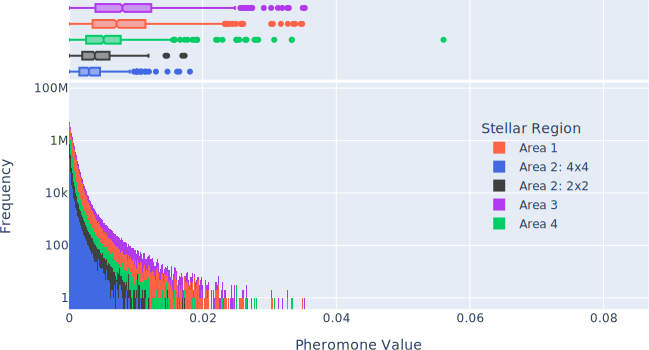
\includegraphics[width=\textwidth,height=6.25cm]{pheromone-plots/pheromone-plot-run-01.pdf}
        \caption{Pheromone Histogram}
    \end{subfigure}
    \begin{subfigure}[b]{0.49\textwidth}
        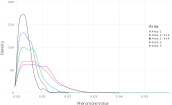
\includegraphics[width=\textwidth,height=6.25cm]{pheromone-plots/pheromone-plot-proportional-run-01.pdf}
        \caption{Pheromone Density Plot}
    \end{subfigure}
    \caption{\label{fig:pheromone-run-1} Plots of Pheromone Values for Experiment 1}
\end{figure}
\begin{figure}[H]
    \centering

    \begin{subfigure}[b]{0.49\textwidth}
        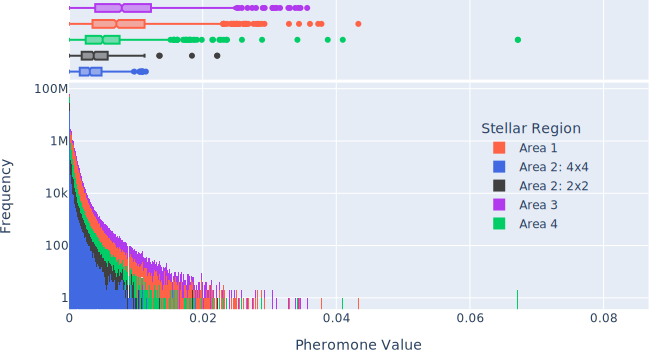
\includegraphics[width=\textwidth,height=6.25cm]{pheromone-plots/pheromone-plot-run-02.pdf}
        \caption{Pheromone Histogram}
    \end{subfigure}
    \begin{subfigure}[b]{0.49\textwidth}
        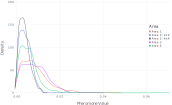
\includegraphics[width=\textwidth,height=6.25cm]{pheromone-plots/pheromone-plot-proportional-run-02.pdf}
        \caption{Pheromone Density Plot}
    \end{subfigure}
    \caption{\label{fig:pheromone-run-2} Plots of Pheromone Values for Experiment 2}
\end{figure}
\begin{figure}[H]
    \centering

    \begin{subfigure}[b]{0.49\textwidth}
        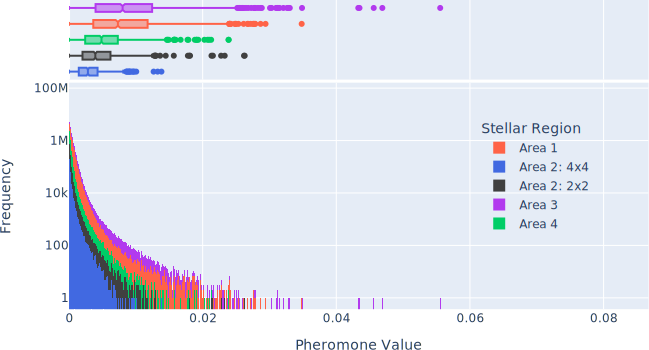
\includegraphics[width=\textwidth,height=6.25cm]{pheromone-plots/pheromone-plot-run-03.pdf}
        \caption{Pheromone Histogram}
    \end{subfigure}
    \begin{subfigure}[b]{0.49\textwidth}
        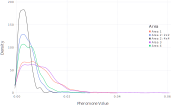
\includegraphics[width=\textwidth,height=6.25cm]{pheromone-plots/pheromone-plot-proportional-run-03.pdf}
        \caption{Pheromone Density Plot}
    \end{subfigure}
    \caption{\label{fig:pheromone-run-3} Plots of Pheromone Values for Experiment 3}
\end{figure}
\begin{figure}[H]
    \centering

    \begin{subfigure}[b]{0.49\textwidth}
        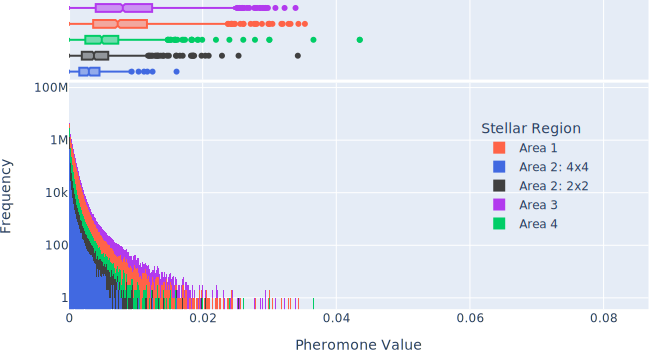
\includegraphics[width=\textwidth,height=6.25cm]{pheromone-plots/pheromone-plot-run-04.pdf}
        \caption{Pheromone Histogram}
    \end{subfigure}
    \begin{subfigure}[b]{0.49\textwidth}
        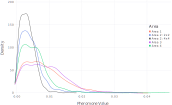
\includegraphics[width=\textwidth,height=6.25cm]{pheromone-plots/pheromone-plot-proportional-run-04.pdf}
        \caption{Pheromone Density Plot}
    \end{subfigure}
    \caption{\label{fig:pheromone-run-4} Plots of Pheromone Values for Experiment 4}
\end{figure}
\begin{figure}[H]
    \centering

    \begin{subfigure}[b]{0.49\textwidth}
        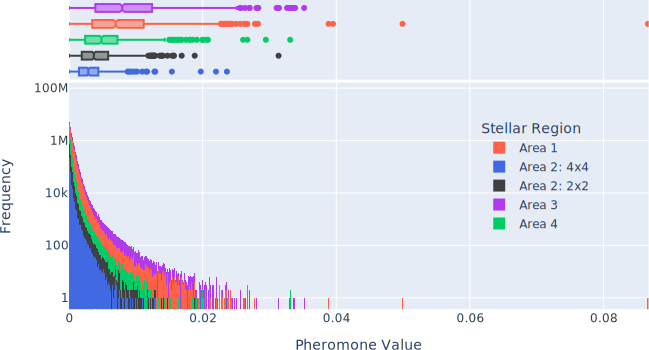
\includegraphics[width=\textwidth,height=6.25cm]{pheromone-plots/pheromone-plot-run-05.pdf}
        \caption{Pheromone Histogram}
    \end{subfigure}
    \begin{subfigure}[b]{0.49\textwidth}
        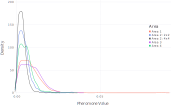
\includegraphics[width=\textwidth,height=6.25cm]{pheromone-plots/pheromone-plot-proportional-run-05.pdf}
        \caption{Pheromone Density Plot}
    \end{subfigure}
    \caption{\label{fig:pheromone-run-5} Plots of Pheromone Values for Experiment 5}
\end{figure}
% Hack to have the geometry of the text on this page look good before the reset on the next page.
\noindent\makebox[\textwidth][c]{%
    \begin{minipage}{6in}
        The distribution of pheromone values across each experiment are similar
        with only minor variations in the outliers present. The bulk of the
        pheromone values lie between 0.00 and 0.01. Area 1 and Area 3
        have similar pheromone distributions despite having a significant difference in
        both their total amount of stars and the amount of stars visited by at least one
        ant. Additionally, Area 2: $\SI{2.0}{\degree}\times\SI{2.0}{\degree}$ has a wider distribution of
        pheromone values than Area 2: $\SI{4.0}{\degree}\times\SI{4.0}{\degree}$.
    \end{minipage}}
\restoregeometry

\section{\label{sec:results-clustering}Gravitational Clustering Based on Pheromone Mapping}
The clustering algorithm is deterministic and so the same input will always result in the same output. However, the clustering directly relies on the results from the Ant Colony. Thus, the clustering phase was also tested across five experiments with each experiment using the results of one of the experiments from the Ant Colony phase.

The results of the clustering phase are sets of stars identified across each raster which constitute the clusters identified within that raster. The raw results detailing the statistics on every cluster identified across every experiment may be seen in Appendix~\ref{sec:appendix} in Tables \ref{tb:results-raw-a1} through Table~\ref{tb:results-raw-a4} and Figures \ref{fig:a1-cluster-overview} through \ref{fig:a4-cluster-overview}. These results were aggregated by combining clusters that overlapped in both their RA bounds and their Dec bounds. Raster plots for these combined results may be seen in Figure~\ref{fig:filtered-clustering-rasters}.

\begin{figure}[H]
    \centering
    \begin{subfigure}[b]{0.75\textwidth}
        \includegraphics[width=\textwidth, height=6cm]{rasters/overlay/area-1-clustering.pdf}
        \caption{\label{fig:clustering-a1-overview}A1}
    \end{subfigure}

    \begin{subfigure}[b]{0.49\textwidth}
        \includegraphics[width=\textwidth, height=6cm]{rasters/overlay/area-2-clustering.pdf}
        \caption{\label{fig:clustering-a2-overview}A2: $\SI{2.0}{\degree}\times\SI{2.0}{\degree}$}
    \end{subfigure}
    \begin{subfigure}[b]{0.49\textwidth}
        \includegraphics[width=\textwidth, height=6cm]{rasters/overlay/area-2-4x4clustering.pdf}
        \caption{\label{fig:clustering-a2-4x4-overview}A2: $\SI{4.0}{\degree}\times\SI{4.0}{\degree}$}
    \end{subfigure}

    \begin{subfigure}[b]{0.49\textwidth}
        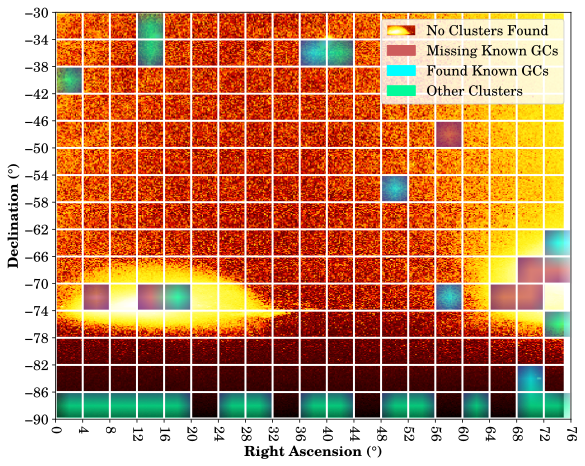
\includegraphics[width=\textwidth, height=6cm]{rasters/overlay/area-3-clustering.pdf}
        \caption{\label{fig:clustering-a3-overview}A3}
    \end{subfigure}
    \begin{subfigure}[b]{0.49\textwidth}
        \includegraphics[width=\textwidth, height=6cm]{rasters/overlay/area-4-clustering.pdf}
        \caption{\label{fig:clustering-a4-overview}A4}
    \end{subfigure}
    \caption{\label{fig:filtered-clustering-rasters}Clustering Raster Classification}
\end{figure}

Similar to the plots for \blobdog{} in Figure~\ref{fig:filtered-dog-rasters}, the results for the clustering have been overlaid on the stellar distribution heat-map for each area. However, while the results for \blobdog{} are simply a binary decision for each raster, the results for the clustering are a set of clusters contained within each raster. Thus, Figure~\ref{fig:filtered-clustering-rasters} does not represent the full results for the clustering and is instead provided to depict the general scope of where known GCs are \textit{Found} or \textit{Missing}, and where \textit{Other Clusters} are detected. It is evident from the figure that a significant amount of the rasters identified contain GCs. The counts for the total number of clusters alongside how many rasters were involved are shown in Table~\ref{tb:clusters-detected-areas}.
\begin{table}[H]
    \centering
    \caption{\label{tb:clusters-detected-areas}Number of Clusters Detected Per Area Across Each Experiment}
    \begin{tabular}{l c@{\hspace{0.1\tabcolsep}}c c@{\hspace{0.1\tabcolsep}}c c@{\hspace{0.1\tabcolsep}}c c@{\hspace{0.1\tabcolsep}}c c@{\hspace{0.1\tabcolsep}}c}
        \toprule
        \multicolumn{1}{c}{\multirow{2}*{Area}}            & \multicolumn{10}{c}{Experiment}                                                                                                                                                                                                                                                                                                                                                                                                                                                                                                                                \\
        \cmidrule(lr){2-11}
                                                           & \multicolumn{2}{c}{1}                                  & \multicolumn{2}{c}{2}                             & \multicolumn{2}{c}{3}                                  & \multicolumn{2}{c}{4}                             & \multicolumn{2}{c}{5}                                                                                                                                                                                                                                                                                                                \\
        \cmidrule(r){1-1} \cmidrule(lr){2-3} \cmidrule(lr){4-5} \cmidrule(lr){6-7} \cmidrule(lr){8-9} \cmidrule(lr){10-11}
                                                           & \multicolumn{1}{C{0.7cm}}{\tiny \# of \mbox{Clusters}} & \multicolumn{1}{C{0.8cm}}{\tiny In \# of Rasters} & \multicolumn{1}{C{0.7cm}}{\tiny \# of \mbox{Clusters}} & \multicolumn{1}{C{0.8cm}}{\tiny In \# of Rasters} & \multicolumn{1}{C{0.7cm}}{\tiny \# of \mbox{Clusters}} & \multicolumn{1}{C{0.8cm}}{\tiny In \# of Rasters} & \multicolumn{1}{C{0.7cm}}{\tiny \# of \mbox{Clusters}} & \multicolumn{1}{C{0.8cm}}{\tiny In \# of Rasters} & \multicolumn{1}{C{0.7cm}}{\tiny \# of \mbox{Clusters}} & \multicolumn{1}{C{0.8cm}}{\tiny In \# of Rasters} \\
        Area 1                                             & 16                                                     & 11                                                & 19                                                     & 13                                                & 18                                                     & 12                                                & 16                                                     & 11                                                & 15                                                     & 10                                                \\
        Area 2: $\SI{2.0}{\degree}\times\SI{2.0}{\degree}$ & 3                                                      & 3                                                 & 1                                                      & 1                                                 & 5                                                      & 5                                                 & 5                                                      & 5                                                 & 3                                                      & 4                                                 \\
        Area 2: $\SI{4.0}{\degree}\times\SI{4.0}{\degree}$ & 0                                                      & 0                                                 & 0                                                      & 0                                                 & 0                                                      & 0                                                 & 0                                                      & 0                                                 & 0                                                      & 0                                                 \\
        Area 3                                             & 27                                                     & 22                                                & 28                                                     & 23                                                & 29                                                     & 24                                                & 29                                                     & 23                                                & 28                                                     & 22                                                \\
        Area 4                                             & 2                                                      & 2                                                 & 2                                                      & 2                                                 & 3                                                      & 3                                                 & 3                                                      & 3                                                 & 1                                                      & 1                                                 \\
        \midrule
        Total                                              & 48                                                     & 38                                                & 50                                                     & 39                                                & 55                                                     & 44                                                & 53                                                     & 42                                                & 47                                                     & 37                                                \\
        \bottomrule
    \end{tabular}
\end{table}

Due to the difference between the number of clusters and the number of involved rasters it is clear that in some cases multiple clusters are found within the same raster. Across the different experiments there is a variety in the number of clusters that were found. However, these differences hover aroud the same ballpark figure, a total of $51\pm4$ clusters. Additionally, across each experiment the arrangement of areas by the number of clusters found remains the same (Area 3 finding the most, followed by Area 1, Area  2: $\SI{2.0}{\degree}\times\SI{2.0}{\degree}$, Area 4, and finally Area 2: $\SI{4.0}{\degree}\times\SI{4.0}{\degree}$). The results compared against the list of known GCs is as follows:
\begin{table}[H]
    \centering
    \caption{Known GCs Detected by Clustering}
    \label{tb:gcs-found-clustering}
    \resizebox{\textwidth}{!}{
        \Large
        \begin{tabular}{l@{\hspace{0.1\tabcolsep}}C{0.2\linewidth}@{\hspace{0.1\tabcolsep}}C{0.2\linewidth}l@{\hspace{0.1\tabcolsep}}C{0.2\linewidth}@{\hspace{0.1\tabcolsep}}C{0.2\linewidth}l@{\hspace{0.1\tabcolsep}}C{0.2\linewidth}@{\hspace{0.1\tabcolsep}}C{0.2\linewidth}}
            \toprule
            \multicolumn{3}{c}{Area 1} & \multicolumn{3}{c}{Area 2} & \multicolumn{3}{c}{Area 3}                                                                                                                                                                                                                       \\
            \cmidrule(lr){1-3} \cmidrule(lr){4-6} \cmidrule(lr){7-9}
            GC                         & Present After Clustering?  & Experiments                                                 & GC  & Present After Clustering? & Experiments                             & GC           & Present After Clustering? & Experiments                                                 \\
            \cmidrule(lr){1-3} \cmidrule(lr){4-6} \cmidrule(lr){7-9}
            Palomar 3                  & No                         & \phantom{1}~\phantom{2}~\phantom{3}~\phantom{4}~\phantom{5} & M71 & Yes                       & 1~\phantom{2}~\phantom{3}~4~\phantom{5} & 47 Tucanae   & No                        & \phantom{1}~\phantom{2}~\phantom{3}~\phantom{4}~\phantom{5} \\
            Willman 1                  & No                         & \phantom{1}~\phantom{2}~\phantom{3}~\phantom{4}~\phantom{5} &     &                           &                                         & NGC 121      & No                        & \phantom{1}~\phantom{2}~\phantom{3}~\phantom{4}~\phantom{5} \\
            Palomar 4                  & No                         & \phantom{1}~\phantom{2}~\phantom{3}~\phantom{4}~\phantom{5} &     &                           &                                         & NGC 362      & No                        & \phantom{1}~\phantom{2}~\phantom{3}~\phantom{4}~\phantom{5} \\
            Koposov 1                  & No                         & \phantom{1}~\phantom{2}~\phantom{3}~\phantom{4}~\phantom{5} &     &                           &                                         & NGC 1049     & Yes                       & 1~2~3~4~5                                                   \\
            NGC 4147                   & Yes                        & 1~2~3~4~5                                                   &     &                           &                                         & NGC 1261     & Yes                       & 1~2~3~4~5                                                   \\
            NGC 5024                   & Yes                        & 1~2~3~4~5                                                   &     &                           &                                         & NGC 1466     & Yes                       & 1~\phantom{2}~3~4~5                                         \\
            NGC 5053                   & Yes                        & 1~2~3~4~\phantom{5}                                         &     &                           &                                         & Arp Madore 1 & No                        & \phantom{1}~\phantom{2}~\phantom{3}~\phantom{4}~\phantom{5} \\
            M3                         & Yes                        & 1~2~3~4~5                                                   &     &                           &                                         & NGC 1629     & No                        & \phantom{1}~\phantom{2}~\phantom{3}~\phantom{4}~\phantom{5} \\
            NGC 5466                   & Yes                        & 1~2~3~4~5                                                   &     &                           &                                         & NGC 1651     & No                        & \phantom{1}~\phantom{2}~\phantom{3}~\phantom{4}~\phantom{5} \\
            Palomar 5                  & Yes                        & 1~2~3~4~5                                                   &     &                           &                                         & NGC 1644     & No                        & \phantom{1}~\phantom{2}~\phantom{3}~\phantom{4}~\phantom{5} \\
            M5                         & Yes                        & \phantom{1}~2~\phantom{3}~\phantom{4}~\phantom{5}           &     &                           &                                         & NGC 1652     & No                        & \phantom{1}~\phantom{2}~\phantom{3}~\phantom{4}~\phantom{5} \\
            GCI 38                     & No                         & \phantom{1}~\phantom{2}~\phantom{3}~\phantom{4}~\phantom{5} &     &                           &                                         & NGC 1841     & Yes                       & 1~2~3~4~5                                                   \\
                                       &                            &                                                             &     &                           &                                         & NGC 1696     & No                        & \phantom{1}~\phantom{2}~\phantom{3}~\phantom{4}~\phantom{5} \\
                                       &                            &                                                             &     &                           &                                         & NGC 1756     & No                        & \phantom{1}~\phantom{2}~\phantom{3}~\phantom{4}~\phantom{5} \\
                                       &                            &                                                             &     &                           &                                         & NGC 1786     & No                        & \phantom{1}~\phantom{2}~\phantom{3}~\phantom{4}~\phantom{5} \\
                                       &                            &                                                             &     &                           &                                         & NGC 1783     & Yes                       & 1~2~3~\phantom{4}~5                                         \\
                                       &                            &                                                             &     &                           &                                         & NGC 1795     & No                        & \phantom{1}~\phantom{2}~\phantom{3}~\phantom{4}~\phantom{5} \\
            \midrule
            Proportion Identified      & {\huge$\nicefrac{7}{12}$}  &                                                             &     & {\huge$\nicefrac{1}{1}$}  &                                         &              & {\huge$\nicefrac{5}{17}$}                                                               \\
            \bottomrule
        \end{tabular}
    }
\end{table}
Most of the GCs that are identified were consistently found across the experiments. The exceptions are the GCs M5 and M71, which were only identified in 1 and 2 experiments respectively. When aggregating the results across all the experiments, the same GCs are discovered in Area 1 and Area 2 as kept by the \blobdog{} filter. However, only 5 of the 17 are identified for Area 3 as compared to 16 of the 17 maintained by \blobdog{}.

\newpage
\section{\label{sec:results-pipeline}Full Pipeline}
The full pipeline constitutes the initial raster filtration by \blobdog{}, followed by the pheromone mapping by the Ant Colony algorithm, which finally culminates in the Gravitational Clustering of the stars based on their pheromone values. This section presents the results of this full pipeline and reframes the results of the previous stages in the context of the full pipeline.
\begin{figure}[H]
    \centering
    \begin{subfigure}[b]{0.75\textwidth}
        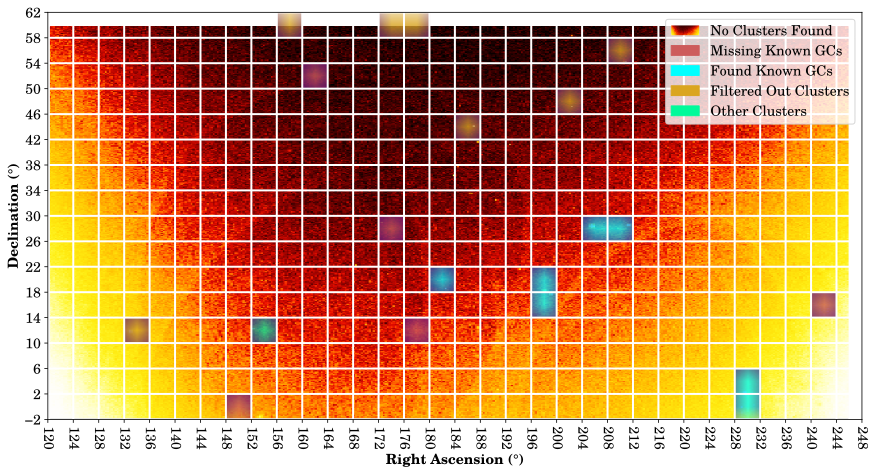
\includegraphics[width=\textwidth, height=6cm]{rasters/overlay/area-1-pipeline.pdf}
        \caption{\label{fig:pipeline-a1-overview}A1}
    \end{subfigure}

    \begin{subfigure}[b]{0.49\textwidth}
        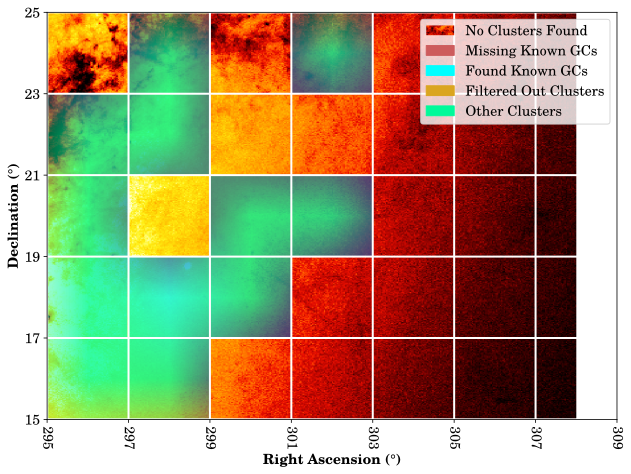
\includegraphics[width=\textwidth, height=6cm]{rasters/overlay/area-2-pipeline.pdf}
        \caption{\label{fig:pipeline-a2-overview}A2: $\SI{2.0}{\degree}\times\SI{2.0}{\degree}$}
    \end{subfigure}
    \begin{subfigure}[b]{0.49\textwidth}
        \includegraphics[width=\textwidth, height=6cm]{rasters/overlay/area-2-4x4pipeline.pdf}
        \caption{\label{fig:pipeline-a2-4x4-overview}A2: $\SI{4.0}{\degree}\times\SI{4.0}{\degree}$}
    \end{subfigure}

    \begin{subfigure}[b]{0.49\textwidth}
        \includegraphics[width=\textwidth, height=6cm]{rasters/overlay/area-3-pipeline.pdf}
        \caption{\label{fig:pipeline-a3-overview}A3}
    \end{subfigure}
    \begin{subfigure}[b]{0.49\textwidth}
        \includegraphics[width=\textwidth, height=6cm]{rasters/overlay/area-4-pipeline.pdf}
        \caption{\label{fig:pipeline-a4-overview}A4}
    \end{subfigure}
    \caption{\label{fig:filtered-pipeline-rasters}Pipeline Raster Classification}
\end{figure}

Figure~\ref{fig:filtered-pipeline-rasters} combines the results of \blobdog{} and the clustering. It showcases the rasters that contain \textit{Found Known GCs} or contain \textit{Missing Known GCs} as well as \textit{Other Clusters}. In addition, it shows the rasters that the clustering phase would have identified as containing a stellar structure but which were preemptively filtered away by \blobdog{} (\textit{Filtered Out Clusters}).

Table \ref{tb:cluster-removals} describes the clusters that were identified by
the clustering but had been filtered away by \blobdog{}. In Table
\ref{tb:results-aggregated} the remaining clusters that were identified by the
clustering are shown. Additionally, it describes the experiments that the
clusters were identified in. Finally, any cluster whose bounds contained an
existing stellar structure according to Stellarium~\cite{Stellarium} has been
marked with the name of the structure and its type. Clusters that did not
corresponding to an existing stellar structure were given the type of
\textit{Nothing}.

\begin{table}[H]
    \centering
    \caption{\label{tb:cluster-removals}All \blobdog{}'s Cluster Removals}
    \begin{tabular}{l L{4.3cm}@{\hspace{0.25\tabcolsep}} c}
        \toprule
        Type             & Name                                             & Experiments                                       \\
        \addlinespace[2em]
        \midrule[0.5pt]
        \multicolumn{3}{c}{Area 1}                                                                                              \\
        \midrule[0.5pt]
        OC               & Golden-Eye Cluster                               & 1~2~3~4~5                                         \\ % a1_132.0_10.0.cluster.json merged: 5
        Galaxy           & NGC~3286 NGC~3288                                & \phantom{1}~\phantom{2}~\phantom{3}~4~\phantom{5} \\ % a1_156.0_58.0.cluster.json merged: 1
        Galaxy           & NGC~3770 NGC~3795                                & \phantom{1}~2~\phantom{3}~\phantom{4}~\phantom{5} \\ % a1_172.0_58.0.cluster.json merged: 1
        Galaxy           & NGC~3838 PGC~36398 PGC~36585 PGC~36655 PGC~36877 & 1~2~3~4~5                                         \\ % a1_176.0_58.0.cluster.json merged: 5
        Galaxy           & Box Galaxy                                       & 1~2~3~4~5                                         \\ % a1_184.0_42.0.cluster.json merged: 5
        Galaxy           & Whirlpool Galaxy                                 & 1~2~3~\phantom{4}~5                               \\ % a1_200.0_46.0.cluster.json merged: 4
        Galaxy           & Pinwheel Galaxy                                  & 1~2~3~4~5                                         \\ % a1_208.0_54.0.cluster.json merged: 5
        \addlinespace[2em]
        \midrule[0.5pt]
        \multicolumn{3}{c}{Area 3}                                                                                              \\
        \midrule[0.5pt]
        Nothing          & N.A.                                             & 1~2~3~4~5                                         \\ % a3_0.0_-90.0.cluster.json merged: 5
        Galaxy           & PGC 993                                          & \phantom{1}~2~3~4~5                               \\ % a3_4.0_-90.0.cluster.json merged: 4
        Nothing          & N.A.                                             & 1~2~3~4~5                                         \\ % a3_8.0_-90.0.cluster.json merged: 5
        Galaxy           & PGC 3533                                         & 1~2~3~4~5                                         \\ % a3_12.0_-90.0.cluster.json merged: 5
        Galaxy           & PGC 216800                                       & 1~2~3~4~5                                         \\ % a3_12.0_-90.0.cluster.json merged: 5
        Nothing          & N.A.                                             & 1~2~3~4~5                                         \\ % a3_16.0_-90.0.cluster.json merged: 5
        Galaxy           & PGC 5780                                         & 1~2~3~4~5                                         \\ % a3_24.0_-90.0.cluster.json merged: 5
        Nothing          & N.A.                                             & 1~2~3~4~5                                         \\ % a3_28.0_-90.0.cluster.json merged: 5
        Galactic Cluster & Abell 3037                                       & 1~2~3~4~\phantom{5}                               \\ % a3_36.0_-90.0.cluster.json merged: 4
        Nothing          & N.A.                                             & 1~2~3~4~5                                         \\ % a3_40.0_-90.0.cluster.json merged: 5
        Nothing          & N.A                                              & 1~2~3~4~5                                         \\ % a3_48.0_-90.0.cluster.json merged: 5
        Nothing          & N.A.                                             & \phantom{1}~2~3~4~\phantom{5}                     \\ % a3_52.0_-90.0.cluster.json merged: 3
        Nothing          & N.A.                                             & 1~\phantom{2}~3~4~5                               \\ % a3_60.0_-90.0.cluster.json merged: 4
        Nothing          & N.A.                                             & 1~\phantom{2}~3~4~5                               \\ % a3_60.0_-90.0.cluster.json merged: 4
        Nothing          & N.A.                                             & 1~2~3~4~5                                         \\ % a3_68.0_-90.0.cluster.json merged: 5
        Nothing          & N.A.                                             & \phantom{1}~\phantom{2}~\phantom{3}~4~5           \\ % a3_68.0_-90.0.cluster.json merged: 2
        Galactic Cluster & Abell 3333                                       & 1~2~3~4~5                                         \\ % a3_72.0_-90.0.cluster.json merged: 5
        \bottomrule
    \end{tabular}
\end{table}

For Area 1, there were 6 galaxies and 1 OC which was filtered away by \blobdog{}. For Area 3, there were 6 galaxies and 11 clusters that were identified as nothing. The average and maximum bounds across the filtered clusters is as follows:

\begin{table}[H]
    \centering
    \caption{Statistics on the RA Bounds and the Dec Bounds for the Filtered Clusters}
    \begin{tabular}{ l|l|l }
                   & Average                              & Max                                  \\
        \hline
        RA Bounds  & \ang[minimum-integer-digits=2]{1.12} & \ang[minimum-integer-digits=2]{1.88} \\
        \hline
        Dec Bounds & \ang[minimum-integer-digits=2]{0.97} & \ang[minimum-integer-digits=2]{1.55} \\
    \end{tabular}
\end{table}
The RA bounds and the Dec bounds reveal that the clusters that \blobdog{} have a diameter of approximately \ang{1.0}. This is in contrast to the bounds corresponding with the results of the clusters identified by the clustering that were also maintained by \blobdog{}. Additional information on the stellar coordinates of each cluster and their bounds may be found in Table~\ref{tb:extended-blob-removal} in Appendix~\ref{chap:blob-extended}.

\begin{table}[H]
    \centering
    \caption{\label{tb:results-aggregated}Clusters Found in All Experiments}
    \begin{tabular}{l L{5.0cm}@{\hspace{0.25\tabcolsep}} c}
        \toprule
        Type              & Name                     & Experiments                                       \\
        \addlinespace[2em]
        \midrule[0.5pt]
        \multicolumn{3}{c}{Area 1}                                                                       \\
        \midrule[0.5pt]
        Dwarf Galaxy      & Regulus Dwarf Galaxy     & 1~2~3~4~5                                         \\ % a1_152.0_10.0.cluster.json merged: 5
        GC                & NGC 4147                 & 1~2~3~4~5                                         \\ % a1_180.0_18.0.cluster.json merged: 5
        GC                & NGC 5024                 & 1~2~3~4~5                                         \\ % a1_196.0_18.0.cluster.json merged: 9
        GC                & NGC 5053                 & 1~2~3~4~\phantom{5}                               \\ % a1_196.0_14.0.cluster.json merged: 5
        GC                & M3                       & 1~2~3~4~5                                         \\ % a1_204.0_26.0.cluster.json merged: 22
        GC                & NGC 5466                 & 1~2~3~4~5                                         \\ % a1_208.0_26.0.cluster.json merged: 10
        GC                & Palomar 5                & \phantom{1}~\phantom{2}~3~\phantom{4}~\phantom{5} \\ % a1_228.0_-2.0.cluster.json merged: 1
        GC                & M5                       & \phantom{1}~2~\phantom{3}~\phantom{4}~\phantom{5} \\ % a1_228.0_2.0.cluster.json merged: 1
        \addlinespace[2em]
        \midrule[0.5pt]
        \multicolumn{3}{c}{Area 2}                                                                       \\
        \midrule[0.5pt]
        Nothing           & N.A.                     & 1~\phantom{2}~\phantom{3}~\phantom{4}~\phantom{5} \\ % a2_295.0_19.0.cluster.json merged: 1
        Nothing           & N.A.                     & \phantom{1}~\phantom{2}~\phantom{3}~\phantom{4}~5 \\ % a2_295.0_17.0.cluster.json merged: 1
        Nothing           & N.A.                     & \phantom{1}~\phantom{2}~\phantom{3}~\phantom{4}~5 \\ % a2_295.0_17.0.cluster.json merged: 1
        Nothing           & N.A.                     & \phantom{1}~\phantom{2}~3~\phantom{4}~\phantom{5} \\ % a2_295.0_21.0.cluster.json merged: 1
        Nothing           & N.A.                     & \phantom{1}~\phantom{2}~\phantom{3}~4~\phantom{5} \\ % a2_295.0_15.0.cluster.json merged: 1
        Nothing           & N.A.                     & \phantom{1}~\phantom{2}~\phantom{3}~4~\phantom{5} \\ % a2_295.0_21.0.cluster.json merged: 1
        Nothing           & N.A.                     & \phantom{1}~\phantom{2}~3~\phantom{4}~\phantom{5} \\ % a2_295.0_17.0.cluster.json merged: 1
        Molecular Cloud   & LDN~758                  & \phantom{1}~\phantom{2}~3~\phantom{4}~\phantom{5} \\ % a2_295.0_19.0.cluster.json merged: 1
        OC                & NGC~6827                 & \phantom{1}~2~\phantom{3}~\phantom{4}~\phantom{5} \\ % a2_297.0_21.0.cluster.json merged: 1
        Nothing           & N.A.                     & 1~\phantom{2}~\phantom{3}~\phantom{4}~\phantom{5} \\ % a2_297.0_23.0.cluster.json merged: 1
        Nothing           & N.A.                     & \phantom{1}~\phantom{2}~\phantom{3}~4~\phantom{5} \\ % a2_297.0_15.0.cluster.json merged: 1
        Absorption Nebula & LDN~787                  & \phantom{1}~\phantom{2}~\phantom{3}~\phantom{4}~5 \\ % a2_297.0_21.0.cluster.json merged: 1
        GC                & M71                      & 1~\phantom{2}~\phantom{3}~4~\phantom{5}           \\ % a2_297.0_17.0.cluster.json merged: 2
        Nothing           & N.A.                     & \phantom{1}~\phantom{2}~\phantom{3}~\phantom{4}~5 \\ % a2_299.0_17.0.cluster.json merged: 1
        Nothing           & N.A.                     & \phantom{1}~\phantom{2}~\phantom{3}~4~\phantom{5} \\ % a2_299.0_19.0.cluster.json merged: 1
        Nothing           & N.A.                     & \phantom{1}~\phantom{2}~3~\phantom{4}~\phantom{5} \\ % a2_299.0_17.0.cluster.json merged: 1
        Nothing           & N.A.                     & \phantom{1}~\phantom{2}~3~\phantom{4}~\phantom{5} \\ % a2_301.0_19.0.cluster.json merged: 1
        Nothing           & N.A.                     & \phantom{1}~\phantom{2}~\phantom{3}~\phantom{4}~5 \\ % a2_301.0_23.0.cluster.json merged: 1
        \addlinespace[2em]
        \midrule[0.5pt]
        \multicolumn{3}{c}{Area 3}                                                                       \\
        \midrule[0.5pt]
        Galaxy            & String of Pearls         & 1~2~3~4~5                                         \\ % a3_0.0_-42.0.cluster.json merged: 5
        Galaxy            & Southern Pinwheel Galaxy & 1~2~3~4~5                                         \\ % a3_12.0_-38.0.cluster.json merged: 5
        Dwarf Galaxy      & Sculptor Dwarf Galaxy    & 1~2~3~4~5                                         \\ % a3_12.0_-34.0.cluster.json merged: 5
        OC                & NGC 419                  & \phantom{1}~2~\phantom{3}~\phantom{4}~\phantom{5} \\ % a3_16.0_-74.0.cluster.json merged: 1
        GC                & NGC 1049                 & 1~2~3~4~5                                         \\ % a3_36.0_-38.0.cluster.json merged: 7
        Galaxy            & Fornax Dwarf Galaxy      & 1~2~3~4~5                                         \\ % a3_40.0_-38.0.cluster.json merged: 10
        GC                & NGC 1261                 & 1~2~3~4~5                                         \\ % a3_48.0_-58.0.cluster.json merged: 11
        GC                & NGC 1466                 & 1~\phantom{2}~3~4~5                               \\ % a3_56.0_-74.0.cluster.json merged: 4
        GC                & NGC 1841                 & 1~2~3~4~5                                         \\ % a3_68.0_-86.0.cluster.json merged: 5
        OC                & NGC 1777                 & 1~2~3~4~5                                         \\ % a3_72.0_-78.0.cluster.json merged: 5
        GC                & NGC 1783                 & 1~2~3~\phantom{4}~5                               \\ % a3_72.0_-66.0.cluster.json merged: 7
        \addlinespace[2em]
        \midrule[0.5pt]
        \multicolumn{3}{c}{Area 4}                                                                       \\
        \midrule[0.5pt]
        HII region        & NGC 7822                 & 1~2~3~4~\phantom{5}                               \\ % a4_0.0_66.0.cluster.json merged: 4
        Galaxy            & Triangulum Galaxy        & 1~2~3~4~5                                         \\ % a4_20.0_30.0.cluster.json merged: 5
        OC                & Double Cluster           & \phantom{1}~\phantom{2}~3~\phantom{4}~\phantom{5} \\ % a4_32.0_54.0.cluster.json merged: 1
        OC                & NGC 1027                 & \phantom{1}~\phantom{2}~\phantom{3}~4~\phantom{5} \\ % a4_40.0_58.0.cluster.json merged: 1
        \bottomrule
    \end{tabular}
\end{table}
\newpage
This table shows that the full pipeline identifies 13 GCs, 5 OCs, 4 Galaxies, 2 Dwarf Galaxies, a Molecular Cloud~\footnote{A dense region of interstellar gas and dust.}, an Absorption Nebula~\footnote{A very dense region within a molecular cloud whose density obscures the light from stars behind it. These regions are known as stellar nurseries as they have the characteristics permitting the formation of new stars.}, and an Emission Nebula~\footnote{The formation of a young star from an absorption nebula. The gravitational force of the gas and dust causes the region to heat up to the point of emitting light in the visible spectrum.}. In addition, it finds 14 clusters that do not correspond to a known stellar structure. For Areas 1, 3, and 4 most of the clusters are found consistently across the experiments. However, in Area 2 the clusters are only found sporadically, being found in at most two experiments.
\begin{table}[H]
    \centering
    \caption{Statistics on the RA Bounds and the Dec Bounds for the Identified Clusters}
    \begin{tabular}{ l|l|l }
                   & Average                              & Max                                  \\
        \hline
        RA Bounds  & \ang[minimum-integer-digits=2]{0.25} & \ang[minimum-integer-digits=2]{1.03} \\
        \hline
        Dec Bounds & \ang[minimum-integer-digits=2]{0.27} & \ang[minimum-integer-digits=2]{1.07} \\
    \end{tabular}
\end{table}
The statistics on the bounds the clusters that were identified by the full pipeline are substantially lower than the bounds for those filtered away by \blobdog{}. Additional information on the stellar coordinates of each cluster and their bounds may be found in Table~\ref{tb:extended-blob-clusters} in Appendix~\ref{chap:blob-extended}.
